\section{Performance}
\author{Kévin Moreau}


\begin{frame}
	\frametitle{Objectifs}

	\begin{block}{Les tâches à effectuer}
	 \begin{itemize}
      \item Amélioration de la plateforme Aerogear ;
	  \item Amélioration des applications Téléphoniques;
	  \item Création d'un outil de mise en place d'un environnement Dynamease complet;
	  \item Mise en place des outils de mesure de performance.
	 \end{itemize}
	\end{block}

	\begin{block}{Amélioration des Applications téléphoniques}
		\begin{itemize}
			\item Récupération rapide des contacts téléphoniques;
			\item Récupération des images de profil des contacts Dynamease.
		\end{itemize}
	\end{block}

    
\end{frame}

\begin{frame}
	\frametitle{Mise en place de l'outil (1/5) : Cahier des charges}

    \begin{block}{Cahier des charges}
	 \begin{itemize}
	  \item Permettre le démarrage d'un environnement Dynamease;
	  \item Utiliser des bases de données déjà remplies;
	  \item Être utilisé facilement par les employés et consultants Dynamease;
	  \item Utiliser des images Docker
	 \end{itemize}
	\end{block}

\end{frame}

\begin{frame}
	\frametitle{Mise en place de l'outil (2/5) : Docker}

    \begin{block}{Fonctionnement}
	 \begin{itemize}
	  \item Gestion de la vente des licences client :
      \item Gestion de la comptabilité associée
	  \item Liaison avec le fournisseur de numéros téléphoniques.
	 \end{itemize}
	\end{block}

	\begin{block}{Termes importants}
	 \begin{itemize}
	  \item Gestion de la vente des licences client :
      \item Gestion de la comptabilité associée
	  \item Liaison avec le fournisseur de numéros téléphoniques.
	 \end{itemize}
	\end{block}

\end{frame}

\begin{frame}
	\frametitle{Mise en place de l'outil (3/5) : Les données}

    \begin{block}{Cahier des charges}
		Mettre schéma pyramide
	\end{block}

\end{frame}

\begin{frame}
	\frametitle{Mise en place de l'outil (4/5) : Ordre de lancement}

    \begin{center}
	  \begin{figure}
        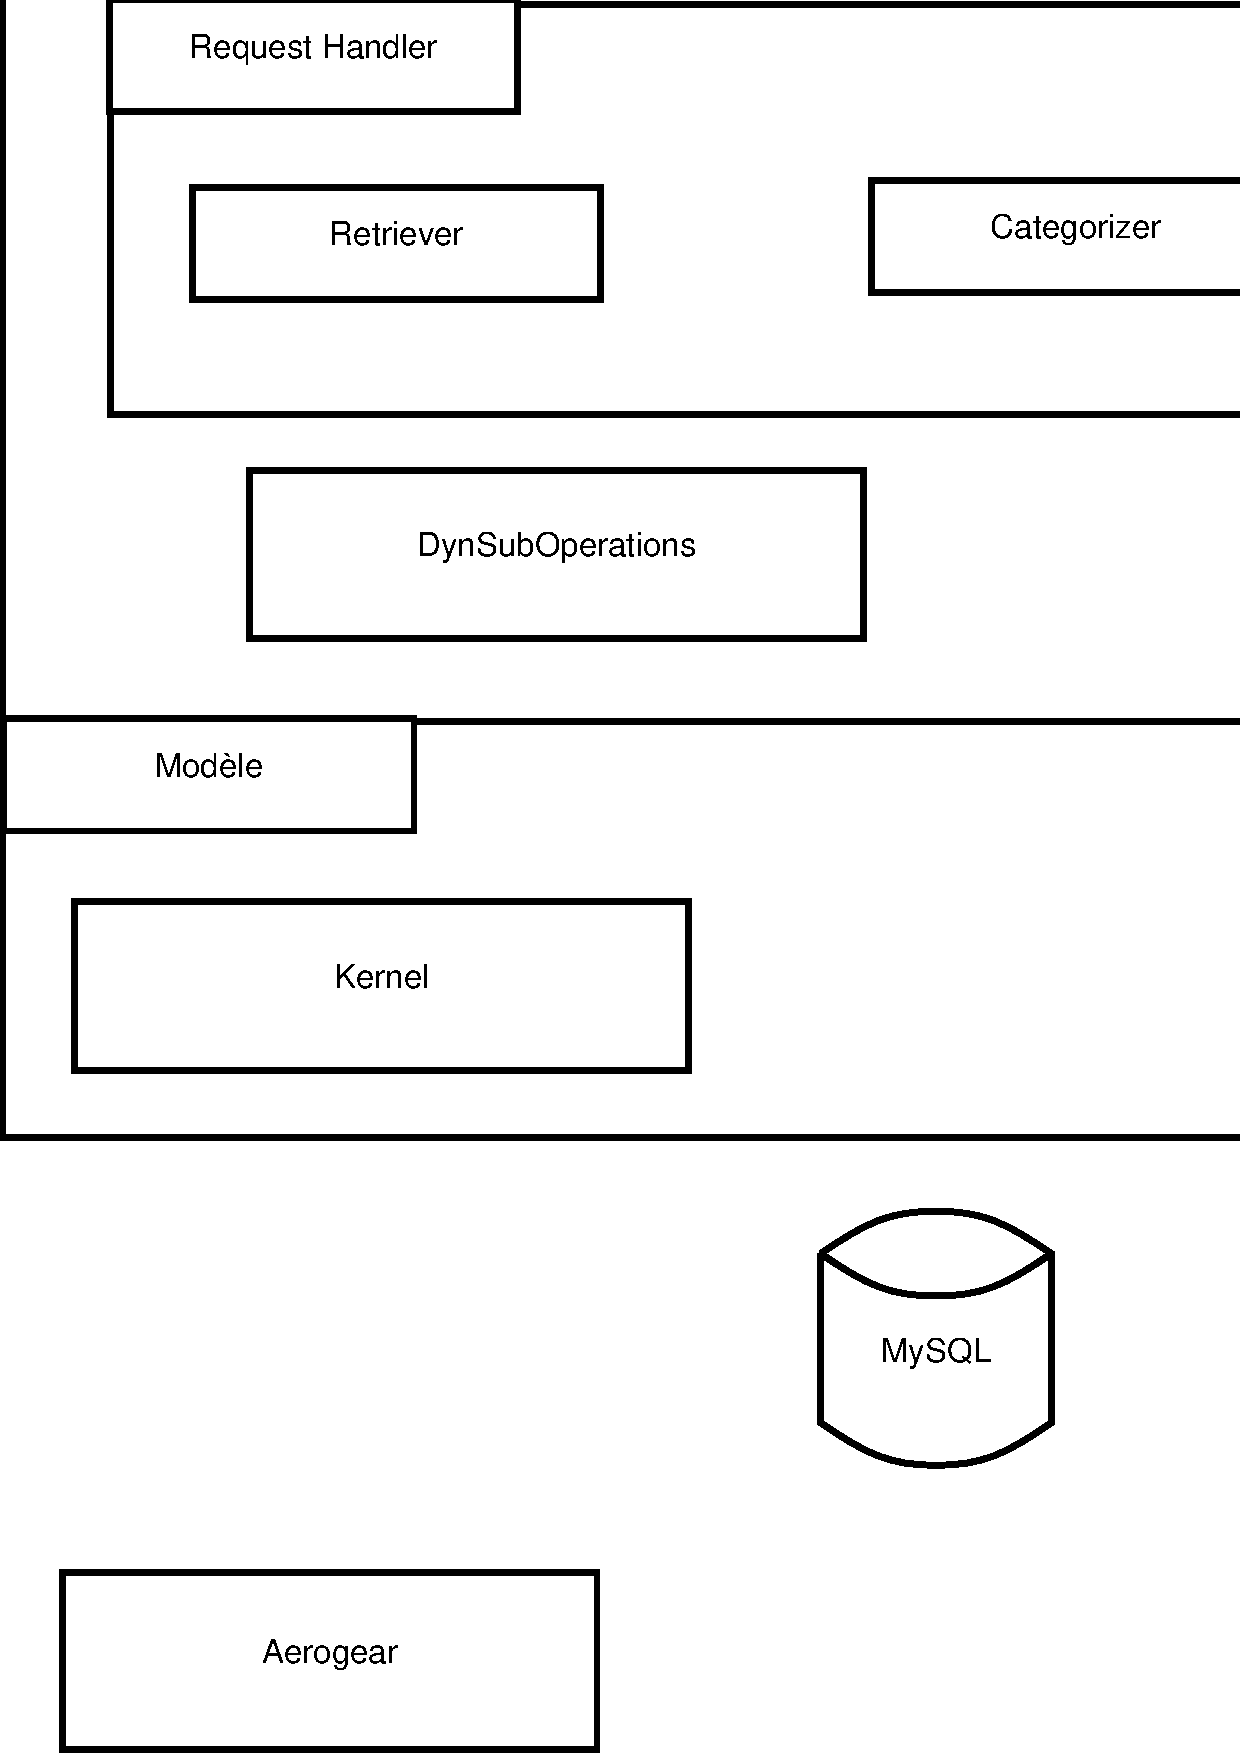
\includegraphics[scale=0.20]{images/pyramide.pdf}
	   \caption{Ordre de lancement des services0}
	  \end{figure}
	\end{center}
\end{frame}


\begin{frame}
	\frametitle{Mise en place de l'outil (5/5) : Fonctionnement}

    \begin{center}
	  \begin{figure}
        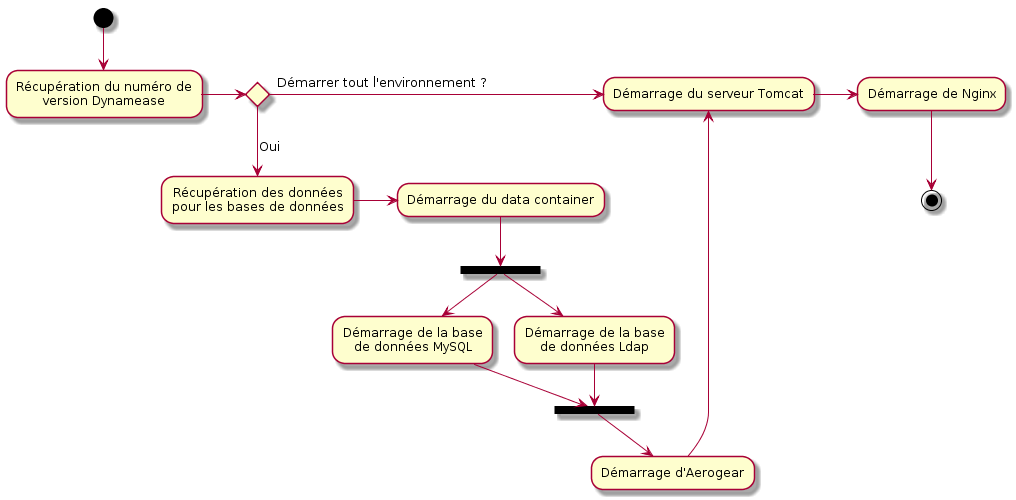
\includegraphics[scale=0.30]{images/activity_outil.png}
	   \caption{Diagramme d'activité du démarrage des services de Dynamease}
	  \end{figure}
	\end{center}

\end{frame}